\documentclass[10pt]{beamer}

\usetheme[progressbar=frametitle]{metropolis}
\usepackage{graphicx}
\usepackage{caption}
\usepackage{appendixnumberbeamer}

\usepackage{booktabs}
\usepackage[scale=2]{ccicons}

\usepackage{pgfplots}
\usepackage{tikz}
\usepgfplotslibrary{dateplot}

\usepackage{xspace}
\newcommand{\themename}{\textbf{\textsc{metropolis}}\xspace}
\usepackage{biblatex}
\bibliography{presentation}
\usepackage{listings}
\usepackage{minted}
\usepackage{verbatim}
\def\b#1{\mathbf{ #1}}
\title{Kernel Independent Fast Multipole and Local Expansions}
\author{\textbf{Isuru Fernando} \\ Acknowledgements: Andreas Kl{\"o}ckner}
% \titlegraphic{\hfill\includegraphics[height=1.5cm]{logo.pdf}}
\usepackage{array}
\newcolumntype{L}{>{\centering\arraybackslash}m{3cm}}
\begin{document}

\maketitle

\begin{frame}[fragile]{Outline}
 \begin{itemize}
  \item Introduction to Multipole and Local expansions
  \item Compressed Taylor Series based Multipole and Local expansions
  \item Results - Accuracy and Time complexity
 \end{itemize}

\end{frame}

\begin{frame}[fragile]{N-body problem}
Let $\b s$ be sources and $\b t$ be targets. Potential at target $\b t_i$ is the sum of all potentials from the sources $\b s$ given by,
\[\psi(\b t, \b s)_i =  \sum_{j} G(t_i, s_j).\]
For example, \[G(t_i, s_j) = \frac{1}{\text{dist}(t_i, s_j)}.\]
\begin{center}
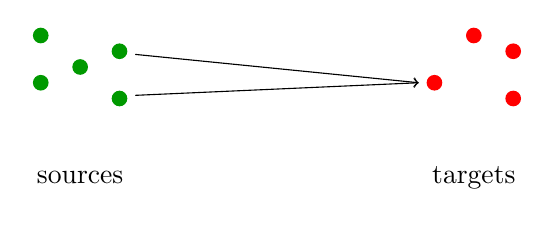
\begin{tikzpicture}[x=1cm,y=0.4cm]
\foreach \Point in {(-2,1.5), (-1,1), (-1.5, 2), (-2,3), (-1,2.5)}{
    \draw \Point node[anchor=center,fill=black!40!green,circle,scale=0.6] {};
}

\foreach \Point in {(3,1.5), (4,1), (3.5,3), (4,2.5)}{
    \draw \Point node[anchor=center,fill=red,circle,scale=0.6] {};
}
\node at (-1.5,-1.5) {sources};
\node at (3.5,-1.5) {targets};

\draw[->] (-0.8,1.1) -- (2.8,1.5);
\draw[->] (-0.8,2.4) -- (2.8,1.5);
\end{tikzpicture}
\end{center}
If the number of sources are $S$ and number of targets are $T$ then,
calculating the potential of all targets takes $\mathcal{O}(S T)$ time.

\end{frame}

\begin{frame}[fragile]{Solving PDEs}
 Some partial differential equations can be turned into an N-body problem.
 For example, \[G(t_i, s_j) = \frac{1}{\text{dist}(t_i, s_j)}.\]
 satisfies,
 \[
  \Delta G(t, s) = \delta(t - s)
 \]
 and therefore,
 \[
  \Delta (G * f) = f(t)
 \]
 which means $G * f$ is a solution to,
 \[
  \Delta u = f
 \]

 Calculating $G * f$ is a N-body problem and therefore solving a partial differential can be reduced to a N-body problem.


\end{frame}


\begin{comment}
\begin{frame}[fragile]{Notation}
Let $p = (p_1, p_2, \ldots p_n)$ be a multi-index where $p_1, p_2, \ldots p_n$ are non-negative integers.

Properties:
\[
 |p| = p_1 + p_2 + \cdots p_n
\]
\[
 p \le q \implies \forall i, p_i \le q_i
\]
\[
 r = p + q \implies \forall i, r_i = p_i + q_i
\]
\[
 x^p = x_1^{p_1} x_2^{p_2} \ldots x_n^{p_n}
\]
\[
 D_x^p = \frac{\partial^{|p|}}{\partial x_1^{p_1} \partial x_2^{p_2} \ldots \partial x_n^{p_n}}
\]
\[
 p! = p_1! p_2! \ldots p_n!
\]
\[
 \binom{p}{q} = \binom{p_1}{q_1} \binom{p_2}{q_2} \cdots \binom{p_n}{q_n}
\]

\end{frame}
\end{comment}

\begin{frame}[fragile]{Local Expansion}
Potential function $\psi(t, s)$ can be written as a Taylor expansion.

\[
 \psi(\b t, \b s) = \sum_{|m| \le p} \underbrace{\frac{D_{\b t}^m \psi(\b t, \b s)\Bigr|_{\b t = \b c}}{m!}}_{\text{depends on src/ctr}} \underbrace{(\b t - \b c)^m}_{\text{depends on tgt/ctr}}
\]
%\begin{align*}
% \sum_{y} \psi(\b x, \b y) &=  \sum_{y} \sum_{|p| \le k} \frac{D_{\b x}^p \psi(\b x, \b y)%\Bigr|_{\b x = \b c}}{p!} (\b x - \b c)^p \\
% &=  \sum_{|p| \le k} \left(\sum_{y} \frac{D_{\b x}^p \psi(\b x, \b y)\Bigr|_{\b x = \b c}}{p!}\right) (\b x - \b c)^p
%\end{align*}
\pause

In 2D, this is,
\begin{align*}
 \psi(\b t, \b s) &= \psi(\b c, \b s) + \psi_x(\b c, \b s)\b h^{(1, 0)} + \psi_y(\b c, \b s)\b h^{(0, 1)} +
\frac{\psi_{xx}(\b c, \b s)}{2!}\b h^{(2, 0)} + \\ & \frac{\psi_{yy}(\b c, \b s)}{2!}(\b c, \b s)\b h^{(0, 2)} + 2 \frac{\psi_{xy}(\b c, \b s)}{2!}(\b c, \b s)\b h^{(1, 1)} + \cdots
\end{align*}

Here,
\[
 \b h^{(a, b)} = (\b t_{[0]}-\b c_{[0]})^a (\b t_{[1]}-\b c_{[1]})^b 
\]

\end{frame}

\begin{frame}[fragile]{Local Expansion}

Coefficients can be computed in $\mathcal{O}(S p^d)$ time where $p$ is the order of the Taylor series and $d$ is the number of dimensions.

Sum can be calculated in $\mathcal{O}(T p^d)$ time.

Cost of the algorithm is $\mathcal{O}(S p^d) + \mathcal{O}(T p^d)$ instead of $\mathcal{O}(S T)$ for calculating the interaction directly.

\end{frame}

\begin{frame}[fragile]{Local Expansion}

Error term in Taylor expansion for Laplace 3D is,
\[
 \sum_{|m| = p+1} \frac{D_{\b t}^m \psi(\b t, \b s)\Bigr|_{\b t = \b c'}}{m!} (\b t - \b c)^m
\]
\[
  \approx \sum_{|m| = p+1} K_m \left(\frac{\b t - \b c}{\b s-\b c}\right)^{m}
\]

It's convergent if all sources are outside the circle around targets.

\begin{center}
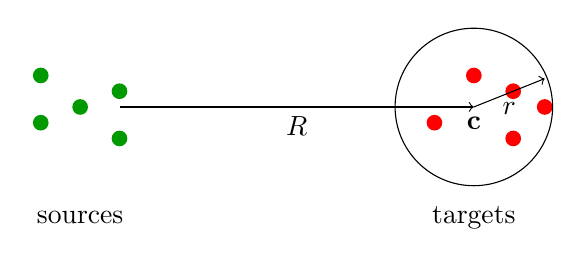
\begin{tikzpicture}[x=1cm,y=0.4cm]

\foreach \Point in {(-2,1.5), (-1,1), (-1.5, 2), (-2,3), (-1,2.5)}{
    \draw \Point node[anchor=center,fill=black!40!green,circle,scale=0.6] {};
}

\foreach \Point in {(3,1.5), (4,1), (3.5,3), (4,2.5), (4.4, 2.0)}{
    \draw \Point node[anchor=center,fill=red,circle,scale=0.6] {};
}

\draw (3.5, 2.0) circle (1cm) node[below] {$\b c$};

\draw[->] (-1,2) -- node[below] {$R$} (3.5,2.0);
\draw[->] (3.5,2.0) -- node[below] {$r$} (4.4,2.9) ;
\node at (-1.5,-1.5) {sources};
\node at (3.5,-1.5) {targets};
\end{tikzpicture}
\end{center}


\end{frame}

\begin{comment}
\begin{frame}[fragile]{Taylor Expansion}

\begin{center}
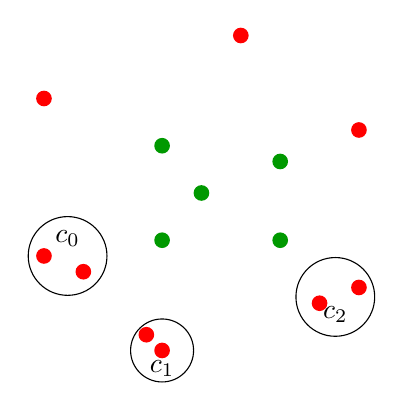
\begin{tikzpicture}[x=1cm,y=0.4cm]
\foreach \Point in {(0,0), (1, 1), (-0.5, -1.5), (-0.5, 1.5), (1.0, -1.5)}{
    \draw \Point node[anchor=center,fill=black!40!green,circle,scale=0.6] {};
}

\foreach \Point in {(-2,-2), (-1.5,-2.5), (-0.5,-5), (-0.7,-4.5), (0.5,5), (-2, 3), (2, -3), (1.5, -3.5), (2, 2)}{
    \draw \Point node[anchor=center,fill=red,circle,scale=0.6] {};
}

\draw (-1.7, -2) circle (0.5cm) node[above] {$\boldsymbol{c}_0$};
\draw (-0.5, -5) circle (0.4cm) node[below] {$\boldsymbol{c}_1$};
\draw (1.7, -3.3) circle (0.5cm) node[below] {$\boldsymbol{c}_2$};
\end{tikzpicture}
\end{center}
Not $\mathcal{O}(S K + K T)$
\end{frame}
\end{comment}

\begin{frame}[fragile]{Multipole Expansion}
Taylor expansion is,
\[
 \psi(\b t, \b s) = \sum_{|m| \le k} \underbrace{\frac{D_{\b t}^m \psi(\b t, \b s)\Bigr|_{\b t = \b c}}{m!}}_{\text{depends on src/ctr}} \underbrace{(\b t - \b c)^m}_{\text{depends on tgt/ctr}}
\]

Changing the variable of differentiation, we get multipole expansion,
\[
 \psi(\b t, \b s) = \sum_{|m| \le k} \underbrace{\frac{D_{\b s}^m \psi(\b t, \b s)\Bigr|_{\b s = \b c}}{m!}}_{\text{depends on tgt/ctr}} \underbrace{(\b s - \b c)^m}_{\text{depends on src/ctr}}
\]
\end{frame}


\begin{frame}[fragile]{Multipole Expansion}

\begin{center}
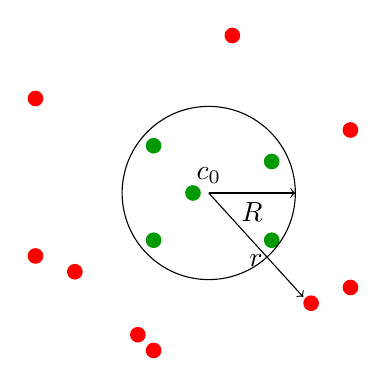
\begin{tikzpicture}[x=1cm,y=0.4cm]
\foreach \Point in {(0,0), (1, 1), (-0.5, -1.5), (-0.5, 1.5), (1.0, -1.5)}{
    \draw \Point node[anchor=center,fill=black!40!green,circle,scale=0.6] {};
}

\foreach \Point in {(-2,-2), (-1.5,-2.5), (-0.5,-5), (-0.7,-4.5), (0.5,5), (-2, 3), (2, -3), (1.5, -3.5), (2, 2)}{
    \draw \Point node[anchor=center,fill=red,circle,scale=0.6] {};
}

\draw (0.2, 0) circle (1.1cm) node[above] {$\boldsymbol{c}_0$};

\draw[->] (0.2,0) -- node[below] {$R$} (1.3,0);
\draw[->] (0.2,0) -- node[below] {$r$} (1.4,-3.3) ;
\end{tikzpicture}
\end{center}

Error for the multipole expansion is \[
  \sum_{|m| = p+1} K_m \left(\frac{\b s - \b c}{\b t-\b c}\right)^{m}
\]
and the expansion is convergent if all targets are outside the circle.
\end{frame}

\begin{frame}[fragile]{Multipole Expansion}

\begin{center}
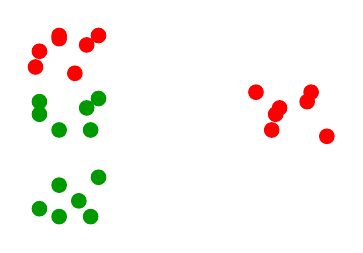
\begin{tikzpicture}[x=1cm,y=0.4cm]


\foreach \Point in {(0.25,0), (1, 1), (0.5, 0.75), (0.75, 0.25), (0.5, -0.25), (0.9, -0.25)}{
    \draw \Point node[anchor=center,fill=black!40!green,circle,scale=0.6] {};
}

\foreach \Point in {(0.25,3), (1.0, 3.5), (0.25, 3.4), (0.85, 3.2), (0.5, 2.5), (0.9, 2.5)}{
    \draw \Point node[anchor=center,fill=black!40!green,circle,scale=0.6] {};
}

\foreach \Point in {(0.25,5), (1.0, 5.5), (0.5, 5.4), (0.85, 5.2), (0.5, 5.5), (0.2, 4.5),(0.7, 4.3)}{
    \draw \Point node[anchor=center,fill=red,circle,scale=0.6] {};
}

\foreach \Point in {(3.25,3), (3.0, 3.7), (3.3, 3.2), (3.65, 3.4), (3.7, 3.7), (3.2, 2.5),(3.9, 2.3)}{
    \draw \Point node[anchor=center,fill=red,circle,scale=0.6] {};
}

%\draw (0.2, 0) circle (1.1cm) node[above] {$\boldsymbol{c}_0$};
%\draw (2.7, 0) circle (1.1cm) node[above] {$\boldsymbol{c}_1$};
%\draw (1.45, 0) circle (2.35cm) node[above] {$\boldsymbol{c}$};

\end{tikzpicture}
\end{center}
\end{frame}

\begin{frame}[fragile]{Multipole Expansion}

\begin{center}
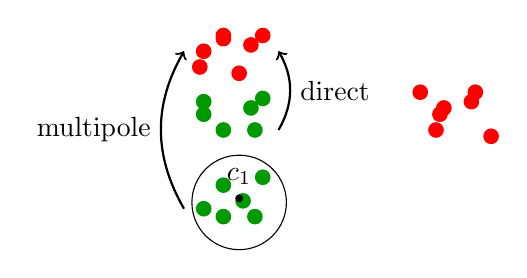
\begin{tikzpicture}[x=1cm,y=0.4cm]


\foreach \Point in {(0.25,0), (1, 1), (0.5, 0.75), (0.75, 0.25), (0.5, -0.25), (0.9, -0.25)}{
    \draw \Point node[anchor=center,fill=black!40!green,circle,scale=0.6] {};
}

\foreach \Point in {(0.25,3), (1.0, 3.5), (0.25, 3.4), (0.85, 3.2), (0.5, 2.5), (0.9, 2.5)}{
    \draw \Point node[anchor=center,fill=black!40!green,circle,scale=0.6] {};
}

\foreach \Point in {(0.25,5), (1.0, 5.5), (0.5, 5.4), (0.85, 5.2), (0.5, 5.5), (0.2, 4.5),(0.7, 4.3)}{
    \draw \Point node[anchor=center,fill=red,circle,scale=0.6] {};
}

\foreach \Point in {(3.25,3), (3.0, 3.7), (3.3, 3.2), (3.65, 3.4), (3.7, 3.7), (3.2, 2.5),(3.9, 2.3)}{
    \draw \Point node[anchor=center,fill=red,circle,scale=0.6] {};
}

\draw[->, thick] (0,0) to [bend left] node[left] {multipole} (0,5);
\draw[->, thick] (1.2,2.5) to [bend right] node[right] {direct} (1.2,5);
%\draw (0.2, 0) circle (1.1cm) node[above] {$\boldsymbol{c}_0$};
%\draw (2.7, 0) circle (1.1cm) node[above] {$\boldsymbol{c}_1$};
\draw (0.7, 0.2) circle (0.6cm) node[above,fill=black,circle,scale=0.3,label=$\boldsymbol{c_1}$] {};

\end{tikzpicture}
\end{center}
\end{frame}

\begin{frame}[fragile]{Multipole Translation}

\begin{center}
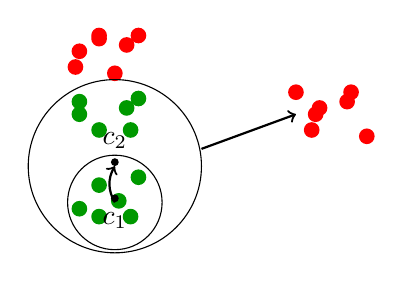
\begin{tikzpicture}[x=1cm,y=0.4cm]


\foreach \Point in {(0.25,0), (1, 1), (0.5, 0.75), (0.75, 0.25), (0.5, -0.25), (0.9, -0.25)}{
    \draw \Point node[anchor=center,fill=black!40!green,circle,scale=0.6] {};
}

\foreach \Point in {(0.25,3), (1.0, 3.5), (0.25, 3.4), (0.85, 3.2), (0.5, 2.5), (0.9, 2.5)}{
    \draw \Point node[anchor=center,fill=black!40!green,circle,scale=0.6] {};
}

\foreach \Point in {(0.25,5), (1.0, 5.5), (0.5, 5.4), (0.85, 5.2), (0.5, 5.5), (0.2, 4.5),(0.7, 4.3)}{
    \draw \Point node[anchor=center,fill=red,circle,scale=0.6] {};
}

\foreach \Point in {(3.25,3), (3.0, 3.7), (3.3, 3.2), (3.65, 3.4), (3.7, 3.7), (3.2, 2.5),(3.9, 2.3)}{
    \draw \Point node[anchor=center,fill=red,circle,scale=0.6] {};
}

\draw[->, thick] (0.7,0.2) to [bend left] node[left] {} (0.7,1.35);
\draw[->, thick] (1.8,1.9) -- node[below] {} (3,3);
%\draw (0.2, 0) circle (1.1cm) node[above] {$\boldsymbol{c}_0$};
%\draw (2.7, 0) circle (1.1cm) node[above] {$\boldsymbol{c}_1$};
\draw (0.7, 0.2) circle (0.6cm) node[above,fill=black,circle,scale=0.3,label=south:$\boldsymbol{c_1}$] {};
\draw (0.7, 1.35) circle (1.1cm) node[above,fill=black,circle,scale=0.3,label=$\boldsymbol{c_2}$] {};

\end{tikzpicture}
\end{center}

Multipole expansion around center $\b c_2$.
\end{frame}

\begin{frame}[fragile]{Compressed Local Expansion forming}
 For eg: 2D Helmholtz equation,
 \[
  \psi_{x x} + \psi_{y y} + \kappa^2 \psi = 0
 \]
 
 We also have,
 \[
  \psi_{x x y} + \psi_{y y y}  + \kappa^2 \psi_y = 0
  \]
  \[
  \psi_{x x x} + \psi_{y y x}  + \kappa^2 \psi_x = 0
 \]
 
 
 
\begin{center}
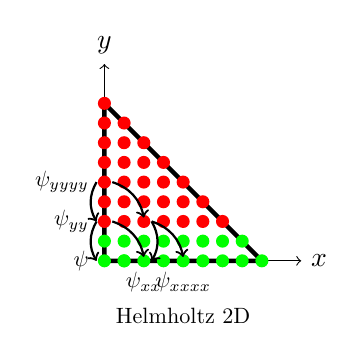
\begin{tikzpicture}[scale=0.5]
\draw[->] (0,0)--(5,0) node[right]{$x$};
\draw[->] (0,0)--(0,5) node[above]{$y$};
\draw[ultra thick] (0,0) node[anchor=north]{}
  -- (4,0) node[anchor=north]{}
  -- (0,4) node[anchor=south]{}
  -- cycle;
  
\foreach \Point in { (0, 0), (0.5, 0), (1.0, 0), (1.5, 0), (2.0, 0), (2.5, 0), (3.0, 0), (3.5, 0), (4.0, 0), (0.5, 0), (0, 0.5), (0.5, 0.5), (1.0, 0.5), (1.5, 0.5), (2.0, 0.5), (2.5, 0.5), (3.0, 0.5), (3.5, 0.5)}{
    \draw \Point node[anchor=center,fill=green,circle,scale=0.5] {};
}

\foreach \Point in { (0.0, 1.0), (0.0, 1.5), (0.0, 2.0), (0.0, 2.5), (0.0, 3.0), (0.0, 3.5), (0.0, 4.0), (0.5, 1.0), (0.5, 1.5), (0.5, 2.0), (0.5, 2.5), (0.5, 3.0), (0.5, 3.5), (1.0, 1.0), (1.0, 1.5), (1.0, 2.0), (1.0, 2.5), (1.0, 3.0), (1.5, 1.0), (1.5, 1.5), (1.5, 2.0), (1.5, 2.5), (2.0, 1.0), (2.0, 1.5), (2.0, 2.0), (2.5, 1.0), (2.5, 1.5), (3.0, 1.0) }{
    \draw \Point node[anchor=center,fill=red,circle,scale=0.5] {};
}

\draw[->, thick] (-0.2,2) to [bend right] node[right] {} (-0.2,1);
\draw[->, thick] (0.2,2) to [bend left] node[right] {} (1,1.1);
\draw[->, thick] (0.2,1) to [bend left] node[right] {} (1,0.1);
\draw[->, thick] (1.2,1) to [bend left] node[right] {} (2,0.1);
\draw[->, thick] (-0.2,1) to [bend right] node[right] {} (-0.2,0);
\draw[->, thick] (1.2,1) to [bend left] node[left] {} (1.2,0);


\node[left,scale=0.8] at (-0.2,0) {$\psi$};
\node[left,scale=0.8] at (-0.2,1) {$\psi_{y y}$};
\node[left,scale=0.8] at (-0.2,2) {$\psi_{y y y y}$};

\node[below,scale=0.8] at (1,-0.1) {$\psi_{x x}$};
\node[below,scale=0.8] at (2,-0.1) {$\psi_{x x x x}$};

\node[below,scale=0.8] at (2,-1) {Helmholtz 2D};

\end{tikzpicture}
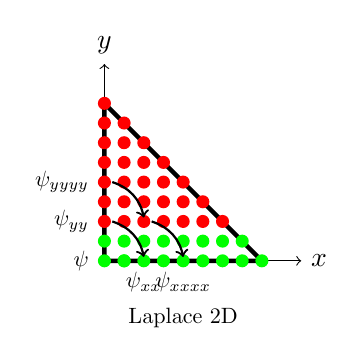
\begin{tikzpicture}[scale=0.5]
\draw[->] (0,0)--(5,0) node[right]{$x$};
\draw[->] (0,0)--(0,5) node[above]{$y$};
\draw[ultra thick] (0,0) node[anchor=north]{}
  -- (4,0) node[anchor=north]{}
  -- (0,4) node[anchor=south]{}
  -- cycle;
  
\foreach \Point in { (0, 0), (0.5, 0), (1.0, 0), (1.5, 0), (2.0, 0), (2.5, 0), (3.0, 0), (3.5, 0), (4.0, 0), (0.5, 0), (0, 0.5), (0.5, 0.5), (1.0, 0.5), (1.5, 0.5), (2.0, 0.5), (2.5, 0.5), (3.0, 0.5), (3.5, 0.5)}{
    \draw \Point node[anchor=center,fill=green,circle,scale=0.5] {};
}

\foreach \Point in { (0.0, 1.0), (0.0, 1.5), (0.0, 2.0), (0.0, 2.5), (0.0, 3.0), (0.0, 3.5), (0.0, 4.0), (0.5, 1.0), (0.5, 1.5), (0.5, 2.0), (0.5, 2.5), (0.5, 3.0), (0.5, 3.5), (1.0, 1.0), (1.0, 1.5), (1.0, 2.0), (1.0, 2.5), (1.0, 3.0), (1.5, 1.0), (1.5, 1.5), (1.5, 2.0), (1.5, 2.5), (2.0, 1.0), (2.0, 1.5), (2.0, 2.0), (2.5, 1.0), (2.5, 1.5), (3.0, 1.0) }{
    \draw \Point node[anchor=center,fill=red,circle,scale=0.5] {};
}

\draw[->, thick] (0.2,2) to [bend left] node[right] {} (1,1.1);
\draw[->, thick] (0.2,1) to [bend left] node[right] {} (1,0.1);
\draw[->, thick] (1.2,1) to [bend left] node[right] {} (2,0.1);

\node[left,scale=0.8] at (-0.2,0) {$\psi$};
\node[left,scale=0.8] at (-0.2,1) {$\psi_{y y}$};
\node[left,scale=0.8] at (-0.2,2) {$\psi_{y y y y}$};

\node[below,scale=0.8] at (1,-0.1) {$\psi_{x x}$};
\node[below,scale=0.8] at (2,-0.1) {$\psi_{x x x x}$};
\node[below,scale=0.8] at (2,-1) {Laplace 2D};

\end{tikzpicture}
\end{center}
\end{frame}


\begin{frame}[fragile]{Compressed Local Expansion forming}
 
 How to do this for any PDE or a system of PDEs?
 
 Let $\b q^{(l)} = (\psi, \psi_{x}, \psi_{y}, \psi_{x x}, \psi_{x y}, \psi_{y y}, \ldots)^T$.
 
 Then from the PDE we can write,
 \[
  \b P \b q^{(l)} = 0
 \]
 \[
  \b q^{(l)} \in \text{Null}(\b P) = \b N
 \]
 $N$ is tall and skinny and therefore $\exists \b M$ s.t.,
 \[
  \b N = \b M \b N_{[\b J, :]}
 \]
 
 We also have,
 \[
  \b q^{(l)} = \b M \b q^{(l)}_{[\b J]}
 \]
 
 Only a subset of $\b q^{(l)}$ needs to be stored and we can use decompression operator $\b M$ to go to full set.
 
 

 \end{frame}
 
\begin{frame}[fragile]{Compressed Local Expansion forming}

 Number of columns in $\b P$ are $\binom{p}{d}$ where $k$ is the order of the Taylor series.

 Number of rows in $\b P$ are $\binom{p-c}{d}$ where $c$ is the order of the PDE.

 From Rank-Nullity theorem,
 \[
  \text{Nullity}(\b P) = \binom{p}{d} - \binom{p-c}{d} = \mathcal{O}(p^{d-1})
 \]

 \[
  \text{size}(\b J) = \text{Rank}(\b N) = \text{Nullity}(\b P) = \mathcal{O}(p^{d-1})
 \]

\end{frame}


\begin{frame}[fragile]{Compressed Multipole Expansion}
 For eg: 2D Helmholtz equation,
 \[
  \psi_{x x} + \psi_{y y} + \kappa^2 \psi = 0
 \]

 Recall, 
 \[
 \psi(\b t, \b s) = \sum_{|m| \le p} \underbrace{\frac{D_{\b s}^m \psi(\b t, \b s)\Bigr|_{\b s = \b c}}{m!}}_{\text{depends on tgt/ctr}} \underbrace{(\b s - \b c)^m}_{\text{depends on src/ctr}}
 \]

 From the PDE we have, 
 \begin{align*}
  c_1 \psi_{x x} +  c_2 \psi_{y y} + c_3 \psi 
  &= c_1 \psi_{x x} +  c_2 (-\psi_{x x} - \kappa^2 \psi) + c_3 \psi \\
  &= (c_1 - c_2) \psi_{x x} + 0 \psi_{y y} +\psi (c_3 - \kappa^2 c_2).
 \end{align*}
\end{frame}

\begin{frame}[fragile]{Compressed Multipole Expansion}
 Let $\b G = (\psi, \psi_{x}, \psi_{y}, \psi_{x x}, \psi_{x y}, \psi_{y y}, \ldots)^T$.

 Let $\b q^{(m)} = (\frac{(\b s - \b c)^{(0, 0)}}{0!}, \frac{(\b s - \b c)^{(1, 0)}}{1!}, \frac{(\b s - \b c)^{(0, 1)}}{1!}, \frac{(\b s - \b c)^{(2, 0)}}{2!}, \frac{(\b s - \b c)^{(1, 1)}}{1!}, \frac{(\b s - \b c)^{(0, 2)}}{2!}, \ldots)^T$.
 
 Then, multipole evaluation is,
 \[
  \b G^T \b q^{(m)} = (\b M \b G_{\b [J]} )^T \b q^{(m)} = ( \b G_{\b [J]} )^T \b M^T \b q^{(m)}
 \]
 
 We can store $\b M^T \b q^{(m)}$ when forming the multipole and this will reduce the complexity of multipole evaluation.

\end{frame}

\begin{frame}[fragile]{Compressed Multipole Expansion}
 $\b M = \mathbb{R}^{p^d \times p^{d-1}}$
 $\implies \b M^T \b q^{(m)} $ is $\mathcal{O}(p^{2d-1})$
 
 Note that $\b P \b M = 0$ and $\b M_{[J, :]}$ is an identity matrix.
 \[
  \b M_{[\bar{J}, :]} = - \b P_2^{-1} \b P_1,
 \]where $\b P_2 = \b P_{[\bar{J}, :]}, \b P_1 = \b P_{[J, :]}$

 $\b P_1, \b P_2$ have $\mathcal{O}(1)$ entries per row and there is a column and row permutation $\b P_2$ of $P_2$ that is triangular.

 Therefore $ \b M^T \b q^{(m)} $ is $\mathcal{O}(p^{d})$
 
\end{frame}





\begin{frame}[fragile]{Compressed Multipole Translation}
Let $\alpha_k = (\b s-\b c_1)^k $ be already computed multipole coefficients around center $\b c_1$. Then,
\begin{align*}
(\b s-\b c)^k &= \left(\left(\b s-\b c_1\right) + \left(\b c_1-\b c\right)\right)^k   \\
&= \sum_{l \le k} \binom{k}{l}\left(\b s-\b c_1\right)^l \left(\b c_1-\b c\right)^{k-l} \\
&= \sum_{l \le k} \beta_{k, l}\left(\b s-\b c_1\right)^l
\end{align*}

Cost: $\mathcal{O}(p^{2d})$
\end{frame}


\begin{frame}[fragile]{Compressed Multipole Translation}

\begin{center}
\vspace*{-2mm}
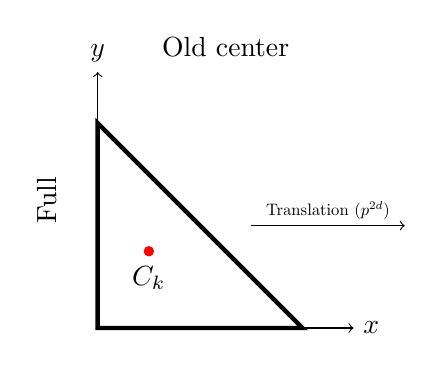
\begin{tikzpicture}[scale=0.65]

\node at (2.5,5.5) {Old center};
\node[rotate=90] at (-1,2.5) {Full};
\draw[->] (0,0)--(5,0) node[right]{$x$};
\draw[->] (0,0)--(0,5) node[above]{$y$};
\draw[ultra thick] (0,0) node[anchor=north]{}
  -- (4,0) node[anchor=north]{}
  -- (0,4) node[anchor=south]{}
  -- cycle;
\draw (1,1.5) node[anchor=center,fill=red,circle,scale=0.4,label=below:$C_k$] {};
\draw[->] (3, 2)-- node[above,scale=0.6]{Translation ($p^{2d}$)} (6,2);
\end{tikzpicture}
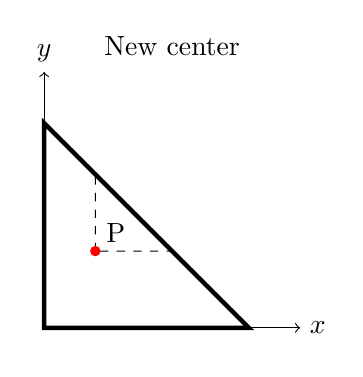
\begin{tikzpicture}[scale=0.65]
\node at (2.5,5.5) {New center};
\draw[->] (0,0)--(5,0) node[right]{$x$};
\draw[->] (0,0)--(0,5) node[above]{$y$};
\draw[ultra thick] (0,0) node[anchor=north]{}
  -- (4,0) node[anchor=north]{}
  -- (0,4) node[anchor=south]{}
  -- cycle;
\draw [dashed] (1,1.5) node[anchor=west]{}
  -- (1,3) node[anchor=north]{}
  -- (2.5,1.5) node[anchor=south]{}
  -- cycle;

\draw (1,1.5) node[anchor=center,fill=red,circle,scale=0.4] {};
\node[color=black] at (1.4,1.85) {P};
%\draw[->] (1,1.5)--(1.4,1.7) node[above]{};
%\draw [dashed,fill=gray] (1.5,1.8) node[fill=black,circle,anchor=center,scale=0.4,label=north:$T_{k+l}$]{};
\end{tikzpicture}

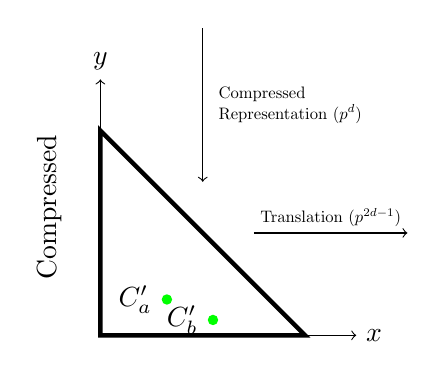
\begin{tikzpicture}[scale=0.65]
\node[rotate=90] at (-1,2.5) {Compressed};
\draw[->] (0,0)--(5,0) node[right]{$x$};
\draw[->] (0,0)--(0,5) node[above]{$y$};
\draw[ultra thick] (0,0) node[anchor=north]{}
  -- (4,0) node[anchor=north]{}
  -- (0,4) node[anchor=south]{}
  -- cycle;
\draw [dashed,fill=gray] (1.3,0.7) node[fill=green,circle,anchor=center,scale=0.4,label=west:$C'_{a}$]{};
\draw [dashed,fill=gray] (2.2,0.3) node[fill=green,circle,anchor=center,scale=0.4,label=west:$C'_{b}$]{};
\draw[->] (3, 2)-- node[above,scale=0.6]{Translation ($p^{2d-1}$)} (6,2);
\draw[->] (2, 6)-- node[right,scale=0.6]{\begin{tabular}{l} Compressed \\ Representation ($p^{d}$) \end{tabular}} (2,3);
\end{tikzpicture}
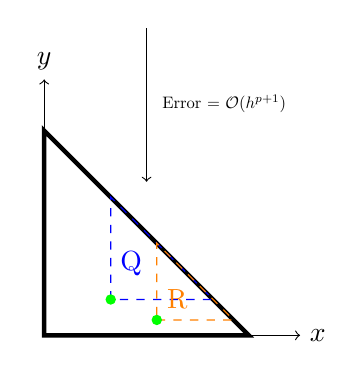
\begin{tikzpicture}[scale=0.65]
\draw[->] (0,0)--(5,0) node[right]{$x$};
\draw[->] (0,0)--(0,5) node[above]{$y$};
\draw[ultra thick] (0,0) node[anchor=north]{}
  -- (4,0) node[anchor=north]{}
  -- (0,4) node[anchor=south]{}
  -- cycle;
\draw [dashed,color=blue] (1.3,0.7) node[anchor=west]{}
  -- (1.3,2.7) node[anchor=north]{}
  -- (3.3,0.7) node[anchor=south]{}
  -- cycle;
\draw [dashed,color=orange] (2.2,0.3) node[anchor=west]{}
  -- (3.7,0.3) node[anchor=north]{}
  -- (2.2,1.8) node[anchor=south]{}
  -- cycle;
\draw [dashed,fill=gray] (1.3,0.7) node {};
\draw [dashed,fill=gray] (2.2,0.3) node {};

\draw [dashed,fill=gray] (1.3,0.7) node[fill=green,circle,anchor=center,scale=0.4]{};
\draw [dashed,fill=gray] (2.2,0.3) node[fill=green,circle,anchor=center,scale=0.4]{};
\node[color=blue] at (1.7,1.4) {Q};
\node[color=orange] at (2.6,0.7) {R};
\draw[->] (2, 6)-- node[right,scale=0.6]{\begin{tabular}{l} Error = $\mathcal{O}(h^{p+1})$ \end{tabular}} (2,3);
%\draw [dashed,fill=gray] (1.8,1.0) node[fill=blue,circle,anchor=center,scale=0.4,label=north:$T'_{a+l}$]{};
%\draw [dashed,fill=gray] (2.7,0.6) node[fill=orange,circle,anchor=center,scale=0.4,label=north:$T''_{b+l}$]{};
%\draw[->] (1.3,0.7)--(1.7,0.9) node[above]{};
\end{tikzpicture}
\end{center}

\end{frame}


\begin{frame}[fragile]{Compressed Multipole and Taylor Expansions}
 
 \begin{table}[]
\begin{tabular}{|L|c|c|c|c|c|c|c|}
\hline & P2L & P2M & M2M & M2L & L2L & L2P & M2P \\ \hline
Taylor Series            & $p^3$     & $p^3$ & $p^{6}$   & $p^{6}$   & $p^{6}$   & $p^{3}$ & $p^{3}$\\ \hline
Compressed Taylor & $p^{2}$ & $p^3$ & $p^{5}$ & $p^{4}$ & $p^{5}$ & $p^{3}$ & $p^{2}$\\ \hline
Laplace ($Y^n_m$ / Point-shoot) & $p^2$ & $p^2$ & $p^3$ & $p^3$ & $p^3$ & $p^2$ & $p^2$\\ \hline
\end{tabular}
  \caption{Time complexities for expansions, translations and evaluations} \label{tab:compressed}
\end{table}

All operations are exact except for M2M in Compressed Taylor.
Point-shoot method uses Spherical Harmonics for expansion instead of a Taylor series. 

Here P is Point, L is Local expansion and M is Multipole expansion.

\end{frame}

\begin{frame}[fragile]{Kernel Independence}
 Point-Shoot method is Laplace specific and requires significant software engineering time for one specific problem.
 
 With Compressed Taylor generating code for Stokes
 \begin{align*} \mu \nabla^2 \mathbf{u} -\boldsymbol{\nabla}p + \mathbf{f} &= \boldsymbol{0} \\
 \boldsymbol{\nabla}\cdot\mathbf{u}&= 0 \end{align*}

 is translated to,
 
 \begin{minted}{python}
    w = make_pde_syms(self.dim, self.dim+1)
    mu = sym.Symbol(self.viscosity_mu_name)
    u = w[:self.dim]
    p = w[-1]
    pdes = (mu * u.laplacian() - p.grad() | u.div())
 \end{minted}

\end{frame}

\begin{frame}[fragile]{Results - Error M2M Stokes}
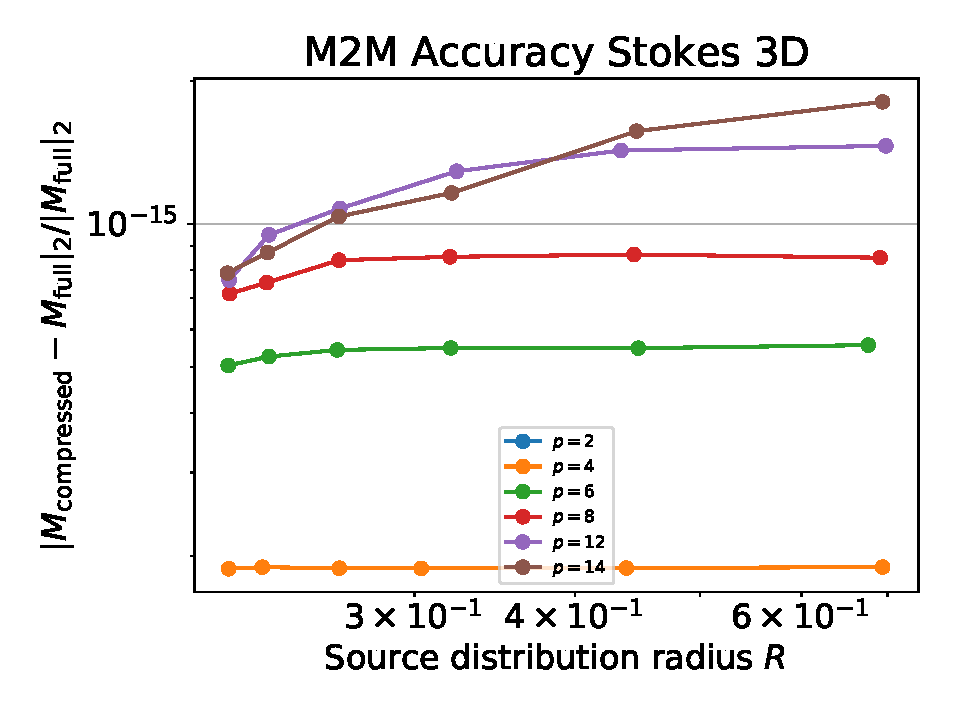
\includegraphics[scale=0.6]{figures/accuracy-stokes-3d.pdf}
\end{frame}

\begin{frame}[fragile]{Results - Error M2M Helmholtz}
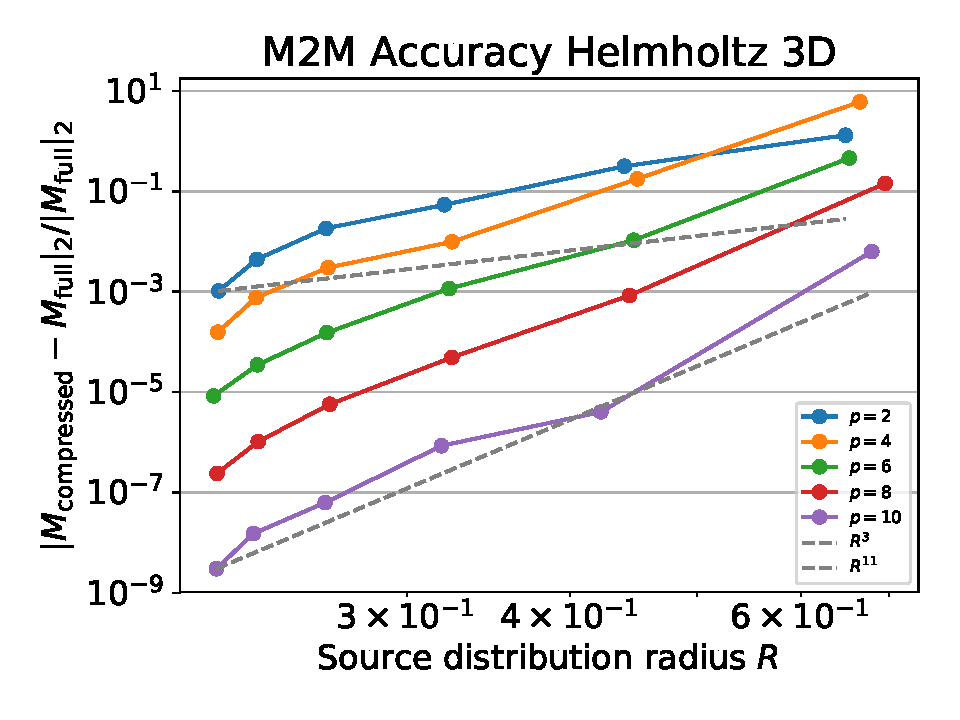
\includegraphics[scale=0.6]{figures/accuracy-helmholtz-3d.pdf}
Credits: Andreas Kl{\"o}eckner, Symbolic Computation for Layer Potential Evaluation with Quadrature by Expansion, CSE 2019
\end{frame}

\begin{frame}[fragile]{Results - FLOP count}
\begin{figure}
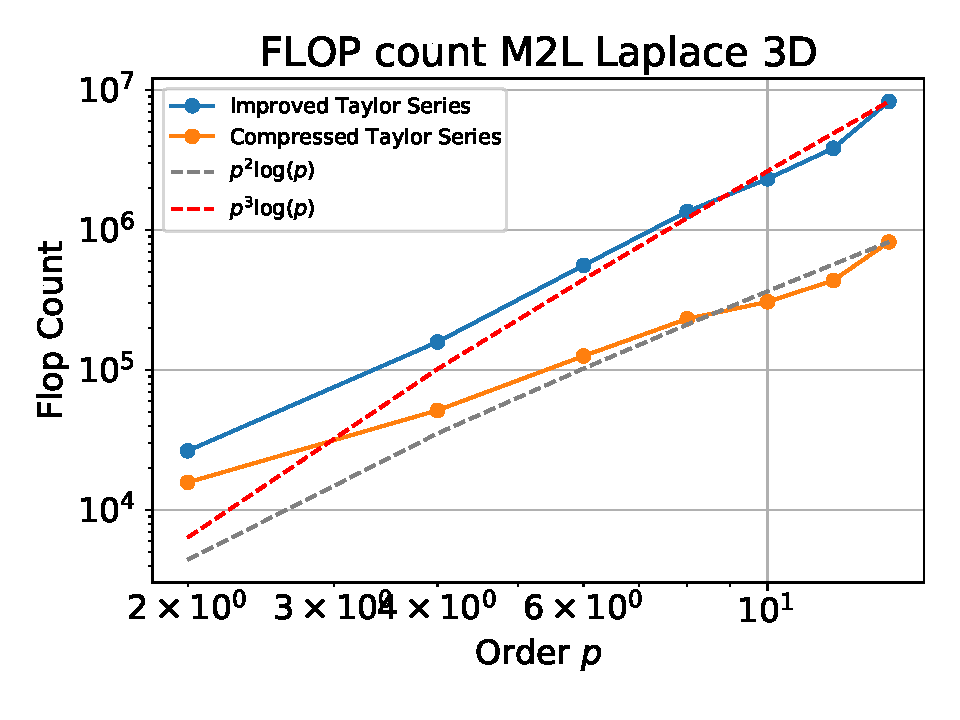
\includegraphics[scale=0.3]{figures/flops-laplace-M2L-3d.pdf}
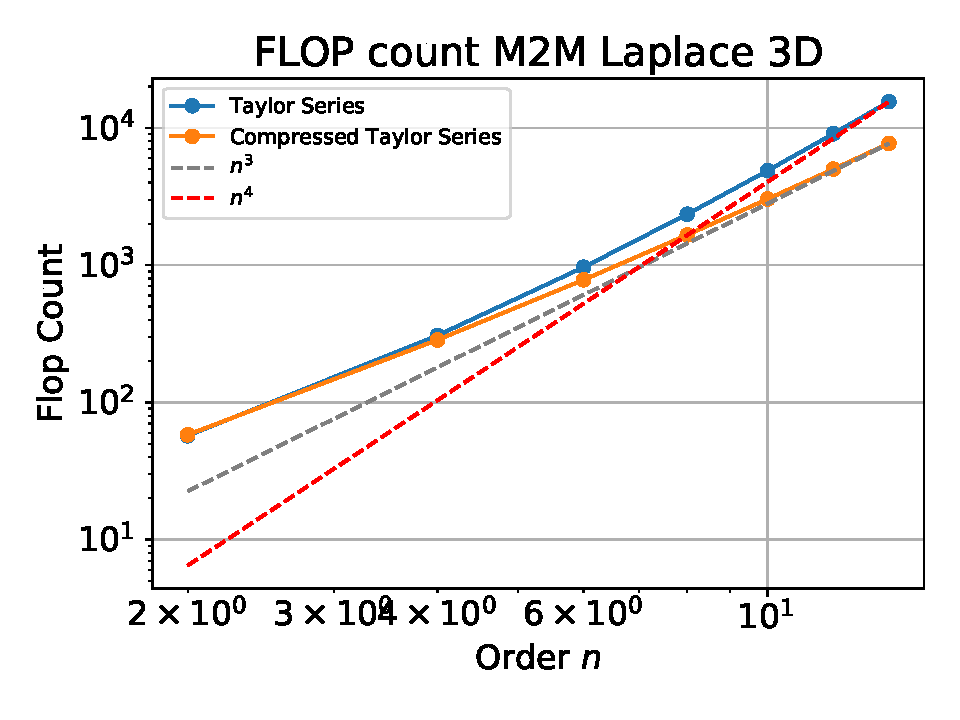
\includegraphics[scale=0.3]{figures/flops-laplace-M2M-3d.pdf}
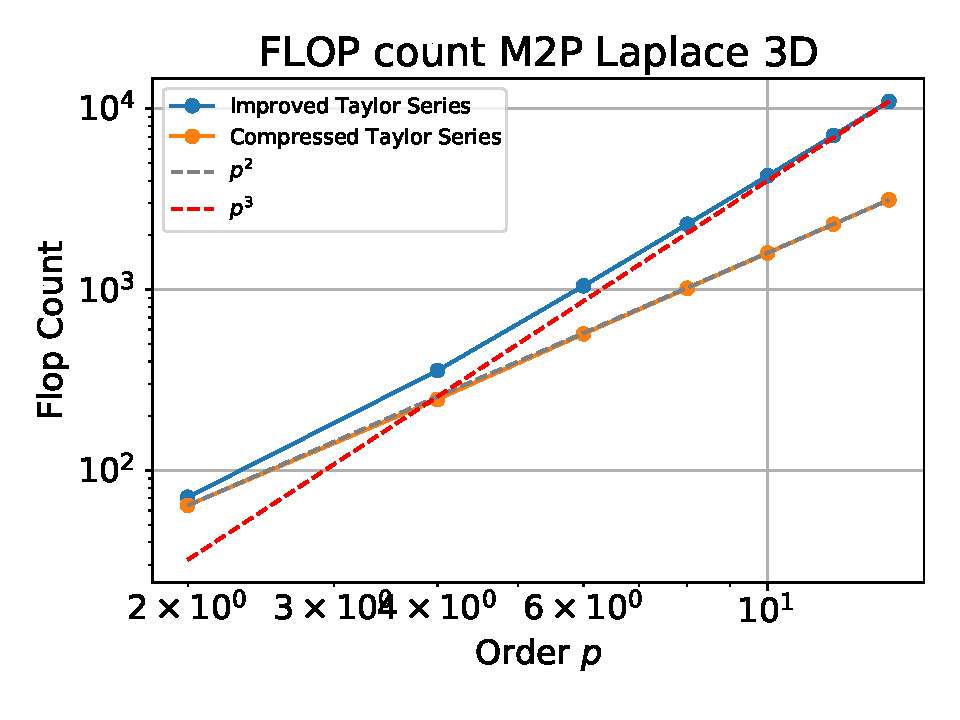
\includegraphics[scale=0.3]{figures/flops-laplace-M2P-3d.pdf}
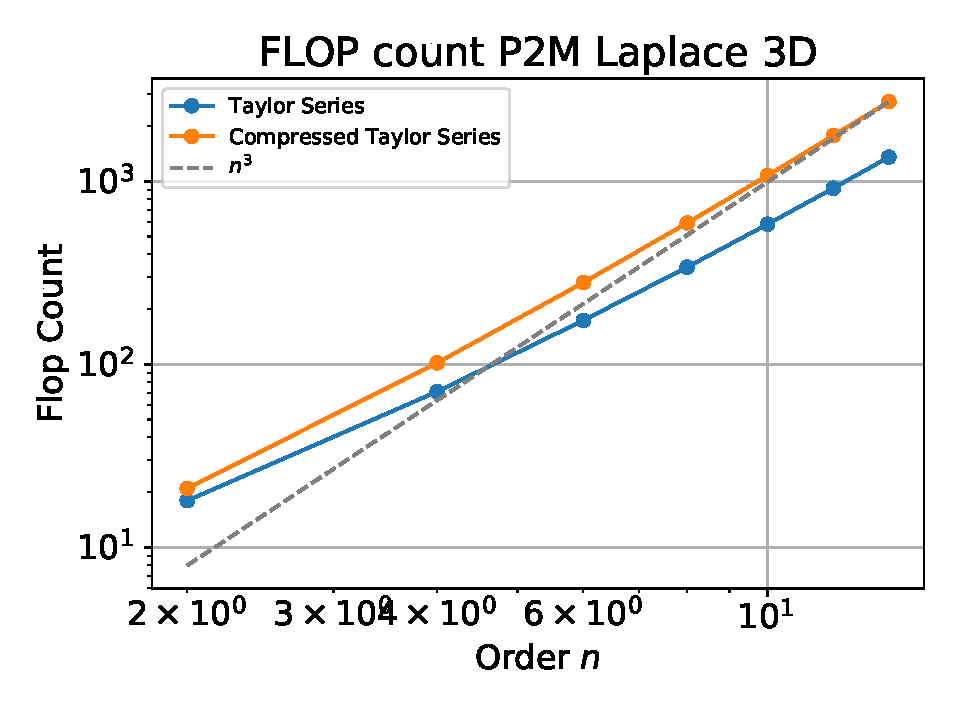
\includegraphics[scale=0.3]{figures/flops-laplace-P2M-3d.pdf}
\end{figure}
\end{frame}

\begin{frame}[fragile]{Conclusions}
\begin{itemize}
 \item Kernel independent method. Only needs the PDE and the Green's function for the PDE.
 \item Asymptotically better than full Taylor Series in,
    \begin{itemize}
     \item Number of FLOPs
     \item Storage
    \end{itemize}
  \item Next goal: A fast Stokes solver on a GPU.
\end{itemize}

\end{frame}

\end{document}

